\section{Promises}

Ein Promise repräsentiert ein Objekt das noch nicht absehbar ist, aber in Zukunft genutzt werden soll. Als Beispiel könnte man den Inhalt einer Datei, die von einem File-Server in einem Browser geladen werden soll, nehmen. Dieser ist auf Anhieb nicht verfügbar, da die Daten zunächst über das Netzwerk übertragen werden müssen. Anstatt auf den Download zu warten, führt der Browser diesen Prozess asynchron aus. Das Prinzip der asynchronen Verarbeitung, bringt dabei Komplexität nach sich. Um dem entgegenzuwirken hat man in dieser Arbeit schon das Prinzip der Callbacks kennengelernt. Dank der Rückruffunktionen ist die Ausführung dieser Sprache in asynchron möglich. Sollten jedoch mehrere asynchrone Events voneinander Abhängig sein, kann das schnell zu unübersichtlichem Code führen (siehe Abb. 9). Mit Promises können voneinander abhängige Events übersichtlich dargestellt werden. Dank der Promise-Verkettung ist es auch möglich Fehlerbehandlungen übersichtlich abzudecken. Während bei Callbacks der Fokus darin liegt, in welcher Reihenfolge die Funktionen aufgerufen werden, sind Promises (mit ECMAScript 2015 eingeführt) danach gerichtet wie man mit dem Ergebnis der Interaktion umgeht.

\subsection{Funktionsweise}

\noindent
Promises \textit{(zu deutsch: Versprechen)} verhalten sich in Javascript ähnlich wie im echten Leben. Die Definition aus dem Wörterbuch ist: Das Versprechen ist eine einseitige Zusage über eine zukünftige Handlung oder ein zukünftiges Ereignis. \cite{versprechen} \\

\noindent
Das heißt:

\begin{enumerate}
    \item Ein Versprechen ist eine Absicherung, dass etwas gemacht wird. Unabhängig davon, ob das Versprechen sich selbst oder von einer anderen Partei gegeben wird.
    
    \item Ein Versprechen kann eingehalten oder gebrochen werden.
    
    \item Wurde ein Versprechen nicht eingehalten, möchte man den Grund für die Nichteinhaltung wissen, um darauffolgend zu handeln.
    
    \item Beim Zeitpunkt eines Versprechens hat man nur die Absicherung. Man kann damit erstmal noch nichts anfangen. Es kann nur geplant werden was nach dem Einhalten des Versprechens gemacht wird. Dementsprechend kann man auch Maßnahmen setzen beim Nichteinhalten dieser Absicherung.
    
\end{enumerate}

\noindent
Dabei gibt es zwei grundlegende Prinzipien der Promises, die zu Verstehen sind: Das \textbf{Erstellen von Promises} und das \textbf{Verarbeiten von Promises}.

\subsubsection{Erstellen eines Promises}

\begin{figure}[H]
\begin{lstlisting}[basicstyle=\small]
new Promise( /* executor */ (resolve, reject) => { ... } );
\end{lstlisting}
\caption{Erzeugung einer neuen Promise-Instanz}
\end{figure}

Der Konstruktor nimmt eine Rückruffunktion als Eingangsparameter. Diese Funktion wird auch \textbf{Executor} genannt.\cite{promise-executor} Der Executor akzeptiert zwei Parameter \textbf{resolve} und \textbf{reject}. Innerhalb dieser Funktion wird eine asynchrone Operation initiiert (z.B. Das suchen einer Datei, eine Datenbankabfrage etc.). Wurde diese asynchrone Operation erfolgreich ausgeführt, ruft der Promise-Konstruktor die resolve Funktion mit dem entsprechendem Ergebnis auf. Anders wird bei einem Fehler die reject Funktion mit der jeweiligen Fehlernachricht aufgerufen. Zur Einführung ein einfaches Beispiel:\\

\noindent
Vor dem Ausführen des Beispiels muss folgend konfiguriert werden:

 \begin{center}
     async-patterns$\,\to\,$ webpack.config.js
 \end{center}

\begin{figure}[H]
\begin{lstlisting}[basicstyle=\small]
module.exports = {
    mode: 'development',
    entry: './src/modules/promises/introduction.ts',
    ...
}
\end{lstlisting}
\end{figure}

\begin{figure}[H]
\begin{lstlisting}[basicstyle=\small]
const keepsHisWord = true;
const resolveRightAway = new Promise((resolve, reject) => {
    if (keepsHisWord) {
        resolve('Promises kept!');
    } else {
        reject('Promise NOT kept!');
    }
});

console.log(resolveRightAway);
\end{lstlisting}
\end{figure}

\noindent
Dieser Promise springt auf Anhieb vom pending in den resolved Zustand, da die abhängige boolean-Variable vorher auf true gesetzt wurde. Umgekehrt, würde die boolean Variable auf false gesetzt werden, würde der Status rejected entsprechen.

\begin{figure}[H]
\centering
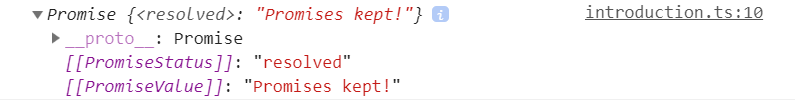
\includegraphics[width=12cm]{promise-beispiel-1}
\caption{Promises haben einen Status und einen Wert}
\end{figure}

\noindent
Der Initialstatus eines Promise wird im nächsten Beispiel verdeutlicht:

\begin{figure}[H]
\begin{lstlisting}[basicstyle=\small]
export interface FakeHttpResponse {
    code: string;
    message: string;
}

const pendingPromise = new Promise<FakeHttpResponse>((resolve, reject) => {
    setTimeout(() => {
        resolve({
            code: '200',
            message: 'Promise kept!'
        });
    }, 10 * 1000);
});

console.log(pendingPromise);
setTimeout(() => console.log(pendingPromise), 10 * 1000);
\end{lstlisting}
\end{figure}

\noindent
Im oberen Beispiel wird der Promise vorbehaltlos nach zehn Sekunden aufgelöst, solange ist der Status ausstehend (pending). Nachdem der Promise aufgelöst wurde, werden Status und Wert aktualisiert. Dabei können nicht nur primitive Typen wie number, boolean oder strings zurückgegeben werden, sondern auch Objekt-Typen und komplexe Typen. Mit anderen Worten: Promises sind generisch.

\begin{figure}[H]
\centering
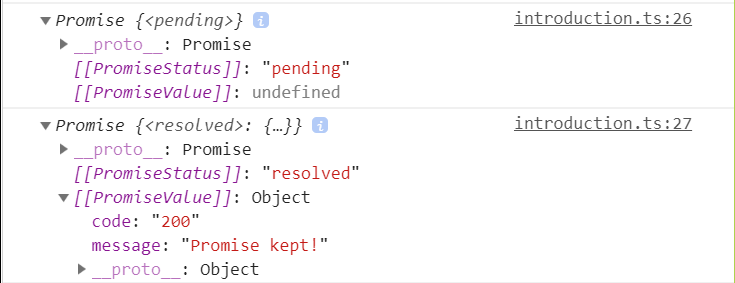
\includegraphics[width=12cm]{promise-beispiel-2}
\caption{Promise hat anfangs den Status \glqq{}ausstehend\grqq{}}
\end{figure}

\noindent
Wie man nun gesehen hat kann ein Promise Objekt den Status  \textbf{pending}, \textbf{resolved} oder \textbf{rejected} haben. Im Status pending ist der Ausgang der Aktion noch ungewiss und deshalb der Promise-Wert undefined. Ändert sich der Status bzw. ist die Aktion zum Promise eingetroffen oder fehlgeschlagen, ist der Status \textbf{settled}. Grundsätzlich läuft ein Promise also vom pending in den settled Status. In der nächsten Sektion wird auf das Verarbeiten von Promises näher eingegangen.

\subsubsection{Verarbeiten von Promises}

Zur Wiederholung: Ein Promise-Objekt repräsentiert das eventuelle Eintreffen oder Fehlschlagen einer asynchronen Operation, einschließlich des entstandenen Wertes. Ein solches Objekt bietet \textbf{statische} Methoden und \textbf{Prototyp}-Methoden. Die statischen Methoden können unabhängig von der Instanz aufgerufen werden, während die Prototyp-Methoden nur mit einer Instanz eines Promise-Objekts aufgerufen werden können. Es gibt drei Prototyp-Methoden. Alle der folgenden Methoden lassen sich unter einem Promise-Event einordnen:

\begin{itemize} 
\item Pending: Der Ausgang des Promises ist noch(!) ungewiss.
\item Resolved: Die Aktion, die zum Promise verlief, ist eingetroffen.
\item Rejected: Die Aktion, die zum Promise verlief, schlug fehl.
\item Settled: Die Aktion ist entweder fehlgeschlagen oder eingetroffen - jedoch abgeschlossen.
\end{itemize}

\noindent
Eine oder mehrere der drei Prototyp-Methoden werden aufgerufen wenn ein Promise in den settled Zustand übergelaufen ist:

\begin{description}

\begin{figure}[H]
\item \begin{lstlisting}[basicstyle=\small]
Promise.prototype.catch(onRejected)
\end{lstlisting}
\end{figure}

\begin{figure}[H]
\item \begin{lstlisting}[basicstyle=\small]
Promise.prototype.then(onFulfilled, onRejected)
\end{lstlisting}
\end{figure}
 
\begin{figure}[H]
\item \begin{lstlisting}[basicstyle=\small]
Promise.prototype.finally(onFinally)
\end{lstlisting}
\end{figure}
 
\end{description}

\noindent
Die untenstehende Grafik zeigt den Ablauf für das Eintreten der Events und wie man diese dann verarbeitet. Mit den Methoden \textbf{then()} und \textbf{catch()} werden auf eintretenden Aktionen reagiert. Da beide Methoden ein neues Promise-Objekt zurückgeben, können Promises reibungslos aneinandergekettet werden. Wenn \textbf{finally} an ein Promise Objekt angebunden wird, wird diese Callback-Funktion in jedem Fall aufgerufen, unabhängig davon ob der Promise \textbf{eingetroffen} oder \textbf{fehlgeschlagen} ist.


\begin{figure}[H]
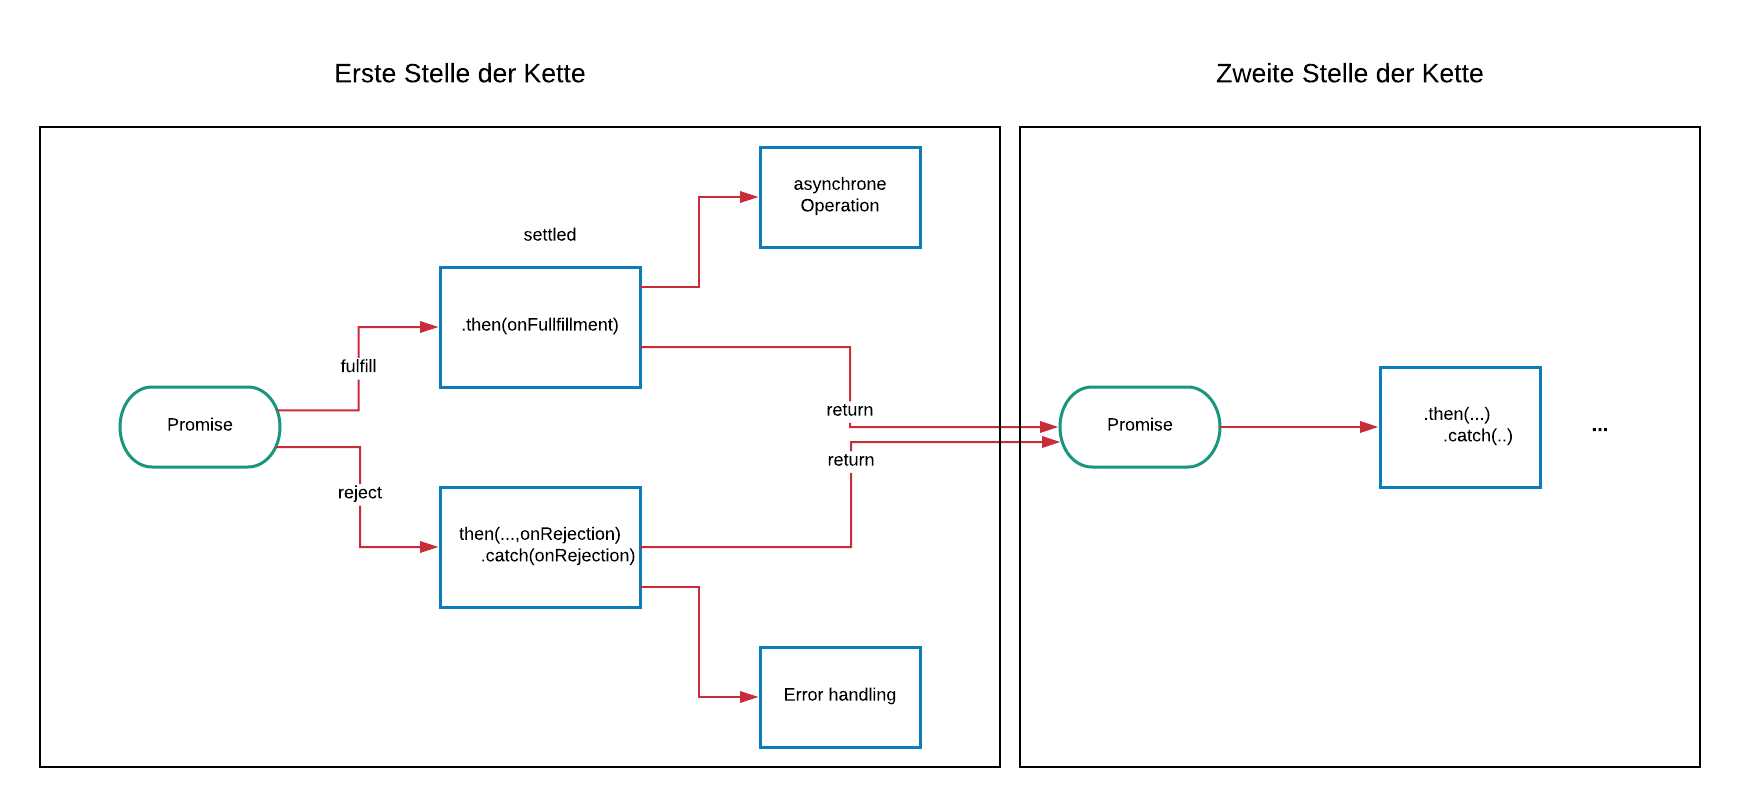
\includegraphics[width=12cm, height=6cm]{Promises-workflow}
\caption{Weiterreichung eines Promise-Objekts \cite{promise-executor}}
\end{figure}

\noindent
Promise-Fehlschläge können dabei auf zwei verschiedene Wege gefangen werden. Innerhalb der then() Methode kann eine zweite Funktion für das \textbf{Nicht-Eintreffen} der Operation festgelegt werden. Ein Beispiel dafür wäre:

\begin{figure}[H]
\begin{lstlisting}[basicstyle=\small]
get('story.json').then((response) => {
  console.log('Success!', response);
}, (error) => {
  console.log('Failed!', error);
})
\end{lstlisting}
\caption{Error-Handling ohne catch. \cite{callback-vs-promises}}
\end{figure}

\begin{figure}[H]
\begin{lstlisting}[basicstyle=\small]
get('story.json').then((response) => {
  console.log('Success!', response);
}).catch((error) => {
  console.log('Failed!', error);
})
\end{lstlisting}
\caption{Error-Handling mit catch. \cite{callback-vs-promises}}
\end{figure}

\noindent
Im Gegensatz zur oberen Variante führt die catch() Methode keine zusätzlichen Operationen aus. Sie macht den Code lediglich semantisch lesbarer. Wichtig zu beachten ist, dass innerhalb einer Executor-Funktion \textbf{niemals} beide Argumente gemeinsam eintreffen können. Sie verhalten sich exklusiv. Deshalb ist das letztere Beispiel im Verhalten vergleichbar mit diesem Beispiel:

\begin{figure}[H]
\begin{lstlisting}[basicstyle=\small]
get('story.json').then((response) => {
  console.log('Success!', response);
}).then(undefined, (error) => {
  console.log('Failed!', error);
})
\end{lstlisting}
\end{figure}

\noindent
Der Unterschied ist minimal, aber extrem hilfreich. Promise-Fehlschläge gelangen bei der nächsten then Methode in den fehlgeschlagen Callback weiter oder in die catch Methode(,wenn vorhanden). Mit then(func1, func2) wird entweder die erste oder die zweite Funktion aufgerufen, aber niemals beide. Jedoch mit then(func1).catch(func2) werden beide Callbacks aufgerufen, sollte die erste Funktion fehlschlagen. Dies ist nur Möglich, da die Funktionen in unterschiedlichen Stellen der Verkettung liegen. Neben den Prototyp-Methoden gibt es, wie bereits erwähnt, die statischen Methoden. Diese bestehen aus vier Methoden:

\begin{itemize}
\item Promise.resolve()
\item Promise.reject()
\item Promise.race()
\item Promise.all()
\end{itemize}

\noindent
Die ersten beiden Methoden werden genutzt um einen eingetroffenen oder fehlgeschlagenen Promises zu simulieren:

\begin{figure}[H]
\begin{lstlisting}[basicstyle=\small]
const rejectedPromise = Promise.reject('I reject on purpose');

rejectedPromise.catch((err: string) => {
    console.log('Reason of failure: ' + err);
});
\end{lstlisting}
\caption{introduction.ts}
\end{figure}

\noindent
Die anderen beiden Methoden helfen Promises leichter zu verarbeiten. Beispielsweise, wenn es darum geht mehrere Promises auszuführen, hat man entweder die Wahl die Promise-Verkettung zu nutzen oder die Promises in einem Array zu lagern und dann die nötigen Aktionen mit der Sammlung von Promises auszuführen. Im nächsten Beispiel wird die \textbf{Promise-Verkettung}, \textbf{Promise.all()} und \textbf{Promise.race()} gegenübergestellt. Vor dem Ausführen des Beispiels muss folgend konfiguriert werden:

 \begin{center}
     async-patterns$\,\to\,$ webpack.config.js
 \end{center}

\begin{figure}[H]
\begin{lstlisting}[basicstyle=\small]
module.exports = {
    mode: 'development',
    entry: './src/modules/promises/stories.ts',
    ...
}
\end{lstlisting}
\end{figure}


\begin{figure}[H]
\begin{lstlisting}[basicstyle=\small]
export class HTTP {

    public makeRequest(url: string): Promise<string> {
        return new Promise((resolve, reject) => {
            const req = new XMLHttpRequest();
            req.open('GET', url);

            req.onload = () => {
                if (req.status === 200) {
                    this.fakeLatency()
                        .then(() => resolve(req.response));
                } else {
                    reject(Error(req.statusText));
                }
            };

            req.onerror = () => {
                reject(Error('Network Error'));
            };

            req.send();
        });
    }

    private fakeLatency() {
        return new Promise((resolve) =>
            setTimeout(resolve, 3000 * Math.random()));
    }
}
\end{lstlisting}
\end{figure}

\begin{figure}[H]
\begin{lstlisting}[basicstyle=\small]
class Story extends HTTP {

    public static BASE_URL = 'https://jsonplaceholder.typicode.com/';

    constructor() {
        super();
    }

    public getAllStories(): Promise<string> {
        const relativeUrl: string = 'posts';
        return this.makeRequest(Story.BASE_URL + relativeUrl);
    }

    public getChapter(chapter: number): Promise<string> {
        return this.makeRequest(`${Story.BASE_URL}posts/${chapter.toString()}`);
    }

    public spawn(result: string | string[]): void {
        const chapter = [];

        if (result instanceof Array === false) {
            chapter.push(JSON.parse(result as string));
        } else {
            for (const post of result) {
                chapter.push(JSON.parse(post));
            }
        }

        chapter.forEach(elm =>
            this.storyElement.innerHTML +=
                `<h1>${elm.title}</h1>
                     <div class="story-info"><i>ID: Post-${elm.id}</i></div>
                 <div><p>${elm.body}.</p></div>`
        );
    }

    public displayFinished(): void {
        document.body.innerHTML += '<div>Done!</div>';
    }

const story = new Story();
\end{lstlisting}
\end{figure}

\noindent
Dieses Beispiel kommt einem praktischen Anwendungsfall relativ nahe. Die Klasse \textbf{HTTP} stellt mit  makeRequest() eine Methode zur Verfügung, die eine Http-Anfrage gegen einen übergebenen Endpunkt macht. Die Methode fakeLatency() simuliert eine Verzögerung der Datenübertragung. Mit der \textbf{Story} Klasse wird zunächst ein Endpunkt für die Datenabfrage definiert. Hierbei handelt es sich um JSONPlaceholder, eine Open Source Endstelle die Beispieldaten für das Prototyping oder zum Testen zur Verfügung stellt. Darüberhinaus werden mit getAllStories() und getChapter() zwei Methoden definiert, die eine Anfrage gegen verschiedene Endpunkte ausführen. Sollte ein Anwendungsfall sein, alle Kapitel anzuzeigen, würde der Code hierfür wie folgt aussehen:

\begin{figure}[H]
\begin{lstlisting}[basicstyle=\small]
story.getAllStories()
    .then((response) => story.spawn(response))
    .finally(() => {
        story.spinnerElement.style.display = 'none';
        story.displayFinished();
    });
\end{lstlisting}
\end{figure}

\noindent
Hier werden zunächst alle Kapitel mit einem einzigen Aufruf am Endpunkt angefragt und daraufhin im Browser abgebildet. Ist der Promise in den settled Zustand angelangt, wird mit finally der Lade-Icon ausgeblendet und eine Nachricht angezeigt, dass alle Stories abgebildet wurden. Sollte jedoch ein Anwendungsfall sein, dass nur drei Stories im Browser angezeigt werden sollen, könnte der Code hierfür so aussehen: 

\begin{figure}[H]
\begin{lstlisting}[basicstyle=\small]
story.getChapter(1).then((response1) => // (*)
    story.spawn(response1)
).then(() => // (**)
    story.getChapter(2).then((response2) => story.spawn(response2))
).then(() => // (***)
    story.getChapter(3).then((response3) => story.spawn(response3))
).finally(() => { // (****)
    story.spinnerElement.style.display = 'none';
    story.displayFinished();
});
\end{lstlisting}
\caption{Promise-Verkettung für sequentielle Ausführungen}
\end{figure}

\noindent
In diesem Fall werden drei Kapitel nacheinander angefragt und im Browser angezeigt. Da die Aufrufe in dem verkettetem Konstrukt voneinander abhängig sind, addiert sich die Zeit die gebraucht wird, um ein Kapitel anzufragen und abzubilden. Die Idee dahinter ist, dass nach jedem Kapitelaufruf und -anzeige gewartet wird, bis diese fertig sind. Der Fluss sieht dabei so aus:

\begin{enumerate}
    \item Das initiale Promise wird aufgerufen und das Kapitel angezeigt
    \item .then() wird aufgerufen und die nächste Sequenz gestartet -         diese endet erst, wenn die Operation innerhalb dieser Methode          erfüllt ist
    \item Das nächste .then() wird initiiert...
\end{enumerate}

Das bedeutet .then() wartet auf die Aktionen innerhalb der Methode.

\begin{figure}[H]
\centering
\includegraphics[width=12cm]{Promise-Verkettung-Stories.png}
\end{figure}

\noindent
Selbst bei einer weiteren Verzögerung der Kapitel innerhalb der Kette, wäre immer noch gewährleistet, dass die Kapitel sequentiell ausgeführt werden:

\begin{figure}[H]
\begin{lstlisting}[basicstyle=\small]
story.getChapter(1).then((response1) => // (*)
    story.spawn(response1)
).then(() => // (**)
    new Promise(resolve => setTimeout(() => resolve(story.getChapter(2)), 5000))
        .then((response2) => story.spawn(response2))
).then() => ...
\end{lstlisting}
\end{figure}

\noindent
Obwohl die voneinander abhängigen Aufrufe in der Darstellung deutlich lesbarer als geschachtelte Callbacks sind, wird mit diesem Beispiel ebenfalls deutlich, dass Promise-Verkettungen den Code in die Länge ziehen können. Da die Kapitel unabhängig voneinander sind (es wird kein Wert innerhalb der Kette weitergereicht), gibt es eine zweite Variante: 

\begin{figure}[H]
\begin{lstlisting}[basicstyle=\small]
const chapters: Array<Promise<void>> = [];

for (const n of [1, 2, 3]) {
    chapters.push(story.getChapter(n));
}

Promise.all(chapters).then((response) =>
    story.spawn(response)
).finally(() => {
    story.spinnerElement.style.display = 'none';
    story.displayFinished();
});
\end{lstlisting}
\caption{Promise.all(iterable) bekommt ein iterierbares Objekt als Parameter übergeben}
\end{figure}

\noindent
Ein Promise.all() kann dabei abhängig vom Übergabeparameter verschiedene Rückgabewerte haben. Sollte das eingegebene iterable Argument leer sein, wird Promise.all() synchron erfüllt. Wenn das eingegebene iterable Argument keine Promises enthält, kommt ein asynchron eingelöstes Promise heraus. In allen anderen Fällen gibt ein Promise.all() ein einzelnes ausstehendes Promise zurück, dass eintrifft wenn alle Promises innerhalb des übergebenen Promise-Arrays eingetroffen sind. Die Rückgabewerte entsprechen dann der Reihenfolge der Promises, unabhängig von der Reihenfolge der Erfüllung.\cite{promise-all}

\noindent
Sollte ein Promise fehlschlagen, wird dieser ebenfalls fehlschlagen mit der Fehlernachricht des ersten fehlgeschlagenen Promise.\cite{promise-executor} Dabei ist zu beachten, dass die Promises parallel voneinander ausgeführt werden.

\begin{figure}[H]
\centering
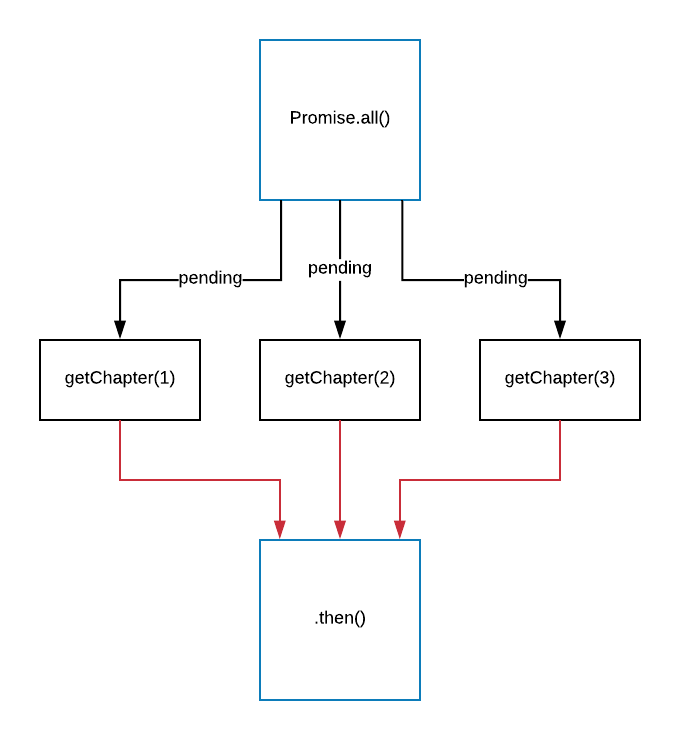
\includegraphics[width=7cm]{promise-all}
\caption{Die Nachrichten werden in der Reihenfolge ausgegeben, in der sie ins Array übergeben worden sind.}
\end{figure}

\noindent
Dagegen wird die nächste Methode verhältnismäßig seltener genutzt. 
Promise.race(iterable) gibt ein erfolgreiches oder fehlgeschlagenes Promise zurück, sobald eines der Promises in dem iterable erfolgreich war oder fehlgeschlagen ist, entsprechend mit dem Wert dieses Promises.
Wenn das übergebene iterable leer ist, wird der Promise für immer im Status pending verharren.\cite{promise-race}

\begin{figure}[H]
\begin{lstlisting}[basicstyle=\small]
Promise.race(chapters).then((response) =>
    story.spawn(response)
).finally(() => {
    story.spinnerElement.style.display = 'none';
    story.displayFinished();
});
\end{lstlisting}
\caption{Es wird nur ein Kapitel mit der Nachricht \glqq Done!\grqq{} angezeigt.}
\end{figure}

\subsection{Anti-Patterns und Best Practices}

Ob bei der Erstellung oder bei der Verarbeitung von Promises - Es gibt gewisse Ansätze nach denen man sich bei der Nutzung richten sollte. Ein negativ Beispiel für die Verarbeitung von Promises, wäre folgendes:

\begin{figure}[H]
\begin{lstlisting}[basicstyle=\small]
story.getChapter(1)
    .then((response1) => {
        story.spawn(response1);
        story.getChapter(2)
            .then((response2) => {
                story.spawn(response2);
                story.getChapter(3).then((response3) => {
                    story.spawn(response3);
                }).finally(() => {
                    story.spinnerElement.style.display = 'none';
                    story.displayFinished();
                });
            });
    });
\end{lstlisting}
\end{figure}

\noindent
Diese Methoden rufen ähnlich wie in Abbildung 17 drei Kapitel nacheinander auf. Obwohl sie im positiv Fall der API-Aufrufe die Kapitel sequentiell laden, wird hier komplett auf den Vorteil, den Promises gegenüber Callbacks bietet, verzichtet. Zudem ist die Ganze Kette davon abhängig, ob der erste Promise-Aufruf eintrifft. Hier wird keinerlei Möglichkeit gewährleistet ein Fehlschlag des ersten Aufrufs zu fangen ohne Code-Duplizierung. Solche ineinandergegliederte Promise-Verschachtelungen werden unter Entwicklern auch als \glqq{}Promise-Hell\grqq{} bezeichnet.
Mit dem ursprünglichen Beispiel (Abb.17) ist es jedoch Möglich Fehler zwischen der Kette zu fangen:

\begin{figure}[H]
\begin{lstlisting}[basicstyle=\small]
story.getChapter(1)
    .then((response1) =>
        story.spawn(response1);
    )
    .catch((err) => ('Catched: ' + err))
    .then(() => story.getChapter(2)
        .then((response2) => 
            story.spawn(response2);
        ))
    ...
    \end{lstlisting}
\end{figure}

\noindent
Als Faustregel für Promises sollte beachtet werden, dass sie nur für einmalig auftretende asynchrone Events genutzt werden sollten. Resolve() wird mit der then() Methode verarbeitet und reject() mit der catch() Methode gefangen. Finally() sollte nur genutzt werden, wenn eine Aktion unabhängig von beiden Events eintreten soll. Der zurückgegebene Typ einer Promise Methode ist immer ein Promise-Objekt, unabhängig davon ob es sich um eine statische- oder einer Prototyp-Methode handelt. Aufgrund dessen lassen sich Promises leicht verketten. Promises bieten mit Promise.all() und Promise.race() Hilfemethoden an, um mehrere Promises leichter zu verarbeiten.




